\chapter{The Mirror World of Investing}

Sooner or later, a person who keeps growing will enter the world of investing.

He may enter through stocks, bonds, funds, business ownership, private companies, real estate, digital assets, or the simple question of what to do with surplus cash. The doorway may differ, but the underlying problem is the same: capital must be placed somewhere, under uncertainty, for the sake of a future result.

Many people postpone this subject with a familiar sentence:

\begin{quote}
When I have money, I will think about investing.
\end{quote}

This sounds reasonable, but it is usually backward. Money is only one ingredient. The harder ingredient is the ability to use money well. That ability takes longer to accumulate than money itself. If a person receives capital before he has learned how capital behaves, the money may simply reveal his ignorance at a larger scale.

So the right attitude is not, ``I have no money, therefore investing has nothing to do with me.'' The right attitude is, ``Because I do not yet have much money, this is the cheapest time to build the judgment required to handle it later.''

Investment education is not only for the wealthy. It is preparation for not being destroyed by wealth, opportunity, or luck when they finally arrive.

\section*{The Formula Is Incomplete Without Luck}

A useful starting formula is:

\[
\text{success} = \text{skill} + \text{luck}.
\]

This formula is simple enough to be dangerous if read lazily. It does not mean every activity contains the same amount of skill and luck. Different domains sit at different places on a spectrum.

At one extreme are activities where skill dominates. Chess and go are close to this side. A stronger player usually beats a weaker player because the rules leave little room for luck.

At the other extreme are activities where luck dominates. A coin toss belongs there. No amount of sincerity, courage, study, or concentration changes the chance of heads on the next throw.

Most human activities sit somewhere in between. Basketball requires skill, but a shot can still roll around the rim and fall out. Business requires skill, but timing, regulation, credit conditions, and accidental encounters matter. Investing requires skill too, but it lives much closer to the luck-heavy side than most clever people want to admit.

\begin{center}
\begin{adjustbox}{max width=\linewidth}
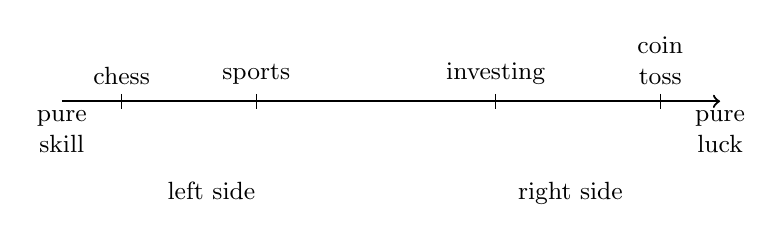
\begin{tikzpicture}[x=0.95cm,y=0.8cm, every node/.style={font=\small, align=center}]
\draw[->, thick] (0,0) -- (8.8,0);
\node[below] at (0,0) {pure\\skill};
\node[below] at (8.8,0) {pure\\luck};

\draw (0.8,0.12) -- (0.8,-0.12);
\node[above] at (0.8,0.12) {chess};

\draw (2.6,0.12) -- (2.6,-0.12);
\node[above] at (2.6,0.12) {sports};

\draw (5.8,0.12) -- (5.8,-0.12);
\node[above] at (5.8,0.12) {investing};

\draw (8.0,0.12) -- (8.0,-0.12);
\node[above] at (8.0,0.12) {coin\\toss};

\node[below=0.9cm] at (2.0,0) {left side};
\node[below=0.9cm] at (6.8,0) {right side};
\end{tikzpicture}
\end{adjustbox}
\end{center}

The diagram is not a final ranking of every activity. It is a way to ask a better question before acting:

\begin{quote}
In this domain, how much of the result is controlled by skill, and how much is exposed to luck?
\end{quote}

That question decides the strategy.

If the activity is mostly skill, then hard practice, repeated correction, visible effort, and more action usually help. If the activity is mostly luck, then more action may not help at all. It may only create more chances to make mistakes.

\section*{Two Mirror Worlds}

The skill-heavy side and the luck-heavy side look like one world from a distance. They are not one world. They are mirror worlds.

In the left-side world, effort often produces visible progress. Practice matters. Discussion helps. Repetition improves performance. The person who acts more, receives more feedback, and corrects faster usually becomes stronger.

In the right-side world, the same behavior may produce the opposite result. More action can mean more transaction cost, more emotional disturbance, more exposure to randomness, and more opportunities for error. A person can work harder and become poorer. He can stare at prices all day and reduce the quality of his decisions. He can collect opinions from a crowd and become less rational than when he began.

\begin{center}
\begin{adjustbox}{max width=\linewidth}
\begin{tabular}{p{0.34\linewidth}p{0.47\linewidth}}
\hline
Left-side strategy & Right-side strategy \\
\hline
Practice frequently. & Prepare before entering. \\
Act, get feedback, correct. & Size positions so waiting is possible. \\
Discuss to reduce error. & Use discussion carefully; uncertainty remains high. \\
Effort after entry improves result. & Most effort should happen before entry. \\
More action often helps. & Less action often protects. \\
\hline
\end{tabular}
\end{adjustbox}
\end{center}

This is why many smart people suffer in investing.

They arrive with strong left-side experience. In school, work, exams, professional skills, and visible competition, they learned that intelligence plus effort plus action usually wins. That experience is real. It should not be despised. But when carried blindly into investing, it becomes dangerous.

A person who has succeeded by action may feel guilty when doing nothing. He wants to adjust, optimize, trade, respond, explain, and improve. In many professions, this impulse is valuable. In investing, it can be fatal.

\section*{The Hardest Action Is Often No Action}

In investing, ``doing nothing'' is not laziness.

It is often the result of work already completed: study, selection, risk control, position sizing, cash-flow planning, and acceptance of uncertainty. Once those decisions have been made well, the best next action may be to wait.

This feels unnatural because most people define effort as visible motion. Studying late for an exam is effort. Writing code is effort. Making sales calls is effort. Practicing a speech is effort. These forms of effort belong mostly to the left-side world.

Investment effort has a different shape.

Before entering, effort means understanding the object, the cycle, the trend, the risk, the sizing, the liquidity, and one's own emotional limits. After entering, effort often means refusing to interfere with a plan merely because fluctuation feels uncomfortable.

\begin{quote}
If an investment requires constant heroic effort after entry, it may have been the wrong investment from the beginning.
\end{quote}

This does not mean one should never review or rebalance. It means that frequent movement should not be confused with competence. In luck-heavy domains, activity can become a costume worn by anxiety.

The investor must learn to ask:

\begin{enumerate}
\item Did new evidence change the thesis?
\item Did my personal risk capacity change?
\item Is this action required by the plan, or by emotion?
\item Am I improving the position, or merely relieving discomfort?
\end{enumerate}

Most unnecessary investment action fails the third question.

\section*{Small Probability Is Not No Probability}

Left-side winners often underestimate small probabilities. They believe that because failure is unlikely, it can be ignored. This is another mirror-world mistake.

A low-probability event can still happen. More importantly, if the loss is large enough, a small probability becomes unacceptable. A \(1\%\) chance of inconvenience is different from a \(1\%\) chance of ruin.

This is why ``never go all in'' is not a timid rule. It is a survival rule.

Consider a simple fair coin. The chance of two unlucky tosses in a row is already \(25\%\). Ten unlucky tosses in a row is rare, but not impossible.

\begin{center}
\begin{adjustbox}{max width=0.78\linewidth}
\begin{tabular}{cc}
\hline
Consecutive losses & Probability \\
\hline
2 & \(25.00\%\) \\
3 & \(12.50\%\) \\
4 & \(6.25\%\) \\
5 & \(3.13\%\) \\
6 & \(1.56\%\) \\
7 & \(0.78\%\) \\
8 & \(0.39\%\) \\
9 & \(0.20\%\) \\
10 & \(0.10\%\) \\
\hline
\end{tabular}
\end{adjustbox}
\end{center}

A person who stakes his whole life on every toss needs only one sufficiently bad sequence to disappear. Skill does not save him if the game design allows ruin.

Risk is not only the volatility of the object. Risk depends on the size of the bet and the size of the bankroll. The same investment can be tolerable for one person and destructive for another. The same decline can be ordinary fluctuation for a properly sized position and a personal catastrophe for an overextended investor.

The practical rule is plain:

\begin{quote}
The more luck a domain contains, the more seriously position size must be controlled.
\end{quote}

\section*{Discussion Also Changes Shape}

In the left-side world, discussion is often powerful. If a problem is mostly governed by stable rules, multiple competent people can examine the same evidence and move toward a better answer. In mathematics, engineering, grammar, accounting, law, programming, and many professional skills, discussion can expose error quickly.

In the right-side world, discussion becomes more difficult.

The uncertainty is higher. The time horizon matters. Risk capacity differs. Information is incomplete. Two people can hold opposite positions and both may have coherent reasons because they are operating with different capital size, obligations, tax situations, time horizons, and psychological endurance.

This does not mean investors should never discuss. It means discussion cannot replace judgment. Crowdsourcing works poorly when each participant is secretly answering a different question.

One person asks, ``Will the price rise next week?''

Another asks, ``Will this asset still matter in ten years?''

Another asks, ``Can I survive a \(50\%\) drawdown?''

Another asks, ``Will this position help me sleep or ruin my family life?''

These are not the same question. Treating them as the same creates noise.

In investing, other people can provide models, warnings, data, and useful disagreement. They cannot donate their risk capacity to you. They cannot live through your volatility for you. They cannot turn your borrowed conviction into real conviction.

\section*{Metacognition at the Border}

The whole point of metacognition is to notice which world you are in.

A rule that works beautifully in one domain may fail in another. A behavior that signals diligence in one context may signal panic in another. A strength in one world may become a weakness in the mirror world.

This is why the most useful answer to many serious questions is:

\begin{quote}
It depends.
\end{quote}

This answer is not evasive when used properly. It is an admission that reality must be located before a rule is applied. The lazy mind wants one universal sentence that works everywhere: work hard, be brave, trust the crowd, never trust the crowd, act fast, be patient, cut losses, hold forever. Each of these may be wise somewhere and foolish somewhere else.

The intelligent question is always: under what conditions?

\begin{center}
\begin{adjustbox}{max width=\linewidth}
\begin{tikzpicture}[node distance=0.65cm, every node/.style={font=\small, align=center}]
\node[draw, rounded corners, minimum width=2.6cm, minimum height=0.72cm] (observe) {observe\\domain};
\node[draw, rounded corners, minimum width=2.6cm, minimum height=0.72cm, right=of observe] (ratio) {estimate\\skill/luck};
\node[draw, rounded corners, minimum width=2.6cm, minimum height=0.72cm, right=of ratio] (strategy) {choose\\strategy};
\node[draw, rounded corners, minimum width=2.6cm, minimum height=0.72cm, below=of ratio] (review) {review\\result};
\draw[->] (observe) -- (ratio);
\draw[->] (ratio) -- (strategy);
\draw[->] (strategy) |- (review);
\draw[->] (review) -| (observe);
\end{tikzpicture}
\end{adjustbox}
\end{center}

The loop is simple: locate the domain, estimate the skill-luck ratio, choose the corresponding strategy, then review the result without pretending the past was obvious.

This protects the practitioner from two opposite errors. He does not treat skill-heavy work as if it were random fate. He does not treat luck-heavy investment as if effort could command the outcome.

\section*{When Effort Does Pay}

The existence of the mirror world does not make effort useless.

It makes effort more precious, because it teaches us where effort belongs. If you find a domain where effort reliably turns into ability, ability into output, and output into value, pay attention. Such domains are rare enough to deserve serious commitment.

Learning a useful skill is often closer to the left side. Writing, programming, selling, speaking, accounting, negotiation, design, and clear thinking can all improve through repeated practice. The returns may not appear instantly, but the relationship between effort and improvement is far more direct than in a price chart.

That is why one should place the most important attention on improving oneself. Money used to acquire a durable skill may not produce immediate excitement, but it changes the person who makes every future decision. This is capital formation at the level of the individual.

A good division of labor emerges:

\begin{quote}
Give effort to the parts that respond to effort. Give time and risk control to the parts that depend heavily on luck.
\end{quote}

In practical terms, this means: build earning ability, learn useful skills, increase cognitive range, improve judgment, keep records, and create multiple sources of income. Then, when capital is invested, do not demand that luck-heavy assets provide the emotional feedback that only left-side practice can provide.

\section*{Driving on the Other Side}

Entering investing is like moving from a country where traffic keeps right to a country where traffic keeps left. The road still looks like a road. The car still looks like a car. The steering wheel, mirrors, pedals, and signs all seem familiar enough. Yet the familiar environment has been reversed in critical ways.

At the beginning, mistakes feel stupid. The driver reaches for the wrong side, looks in the wrong direction, drifts toward the wrong lane, and almost creates danger precisely because he thinks he already knows how driving works.

That is the danger of the mirror world.

The investor recognizes words he has seen before: effort, discipline, research, confidence, opportunity, risk, action, patience. But many of them have changed meaning. Discipline may mean not trading. Confidence may mean smaller sizing. Research may mean deciding not to enter. Opportunity may mean waiting with cash. Patience may mean watching an apparent loss remain apparent for years without forcing a bad exit.

Once this reversal is understood, investing becomes less mystical. The difficulty does not disappear, but it becomes more honest. The question is no longer, ``Why does my intelligence fail here?'' The question becomes, ``Which rule from the other world am I applying in the wrong place?''

A person seeking wealth freedom must learn to move between both worlds.

In the left-side world, work hard, practice deliberately, ask for correction, and increase skill. In the right-side world, respect uncertainty, avoid ruin, size modestly, prepare before acting, and let time do the part that effort cannot do.

Freedom requires both. Skill builds the person. Capital needs time. Metacognition tells you which world you are standing in before you choose how to move.
